\documentclass[a4paper, 12pt]{ctexart}
\usepackage[UTF8]{ctex}
\usepackage{amsmath}
\usepackage{graphicx}
\usepackage{grffile}
\usepackage{longtable}
\usepackage{wrapfig}
\usepackage{rotating}
\usepackage{cases}
\usepackage{mathrsfs}
\usepackage{amssymb} 
\usepackage{amsthm}
\usepackage{xltxtra} 
\usepackage{mflogo,texnames}
\usepackage{indentfirst}
\usepackage[normalem]{ulem}
\usepackage{textcomp}
\usepackage{booktabs}
\usepackage{subfigure}
\usepackage{caption}
\usepackage[linktocpage,pdfstartview=FitH,colorlinks,
linkcolor=blue,anchorcolor=blue,
citecolor=blue,filecolor=blue,menucolor=blue,urlcolor=blue]{hyperref}
\usepackage{setspace,csquotes, enumitem,endnotes,fontspec, capt-of}
\doublespacing
\usepackage[margin=1in]{geometry}
\usepackage[notes, notetype=endonly, isbn=false, backend=biber]{biblatex-chicago}
\bibliography{shiff2016b}
\let\footnote=\endnote
\let\cite=\endnote
\let\footcite=\autocite
\setCJKmainfont{SimSun}
\setmainfont{Calibri} 
\CTEXsetup[format={\Large\bfseries}]{section}
\setlist[enumerate,itemize]{noitemsep,nolistsep,leftmargin=*}
% \newtheorem*{theorem}{解}
% \newtheorem*{example}{问题}
\usepackage{listings}
\usepackage[usenames,dvipsnames]{color}
\definecolor{myblue}{rgb}{0.13, 0.13, 1.0}
\definecolor{mypurple}{rgb}{0.5, 0.0, 0.5}
\lstset{
    language=Python,
    basicstyle=\small,
    keywordstyle=[1]\color{myblue}\bfseries,   % keywords in bold blue
    keywordstyle=[2]\color{mypurple},          % function arguments in purple
    keywordstyle=[3]\color{myblue}\underbar,   % user-defined functions in blue with underbar
    stringstyle=\color{mypurple},              % strings in purple
    showstringspaces=false,
    identifierstyle=,
    tabsize=4,
    morekeywords={sawtooth, square},           % additional keywords
    morekeywords=[2]{on, off, interp},         % additional function arguments
    morekeywords=[3]{FindESS, homework_example},% user-defined functions
    morecomment=[l][\color{myblue}]{...},      % line continuation (...) like blue comment
    numbers=left,
    numberstyle=\tiny\color{myblue},
    firstnumber=1,
    stepnumber=1
}


\author{张天骏 \\ 2021300003004}
\date{}
\title{“Finance and Development: A Tale of Two Sectors” \ 论文复现  \\  \large《递归宏观经济学》结课论文}



\begin{document}
\maketitle

% \newpage
% \tableofcontents   

\section{论文模型简介}
这篇论文建立了一个包含两个部门的经济模型,S (规模较小,服务业)和m(规模大,制造业多)。服务业部门的产出仅用于消费。制成品用于消费和投资,是计价物。
假设社会中存在无限生命的个体,总测度为1,这些个体在财富和创业想法或天赋的质量上是异质的。这部分由随机向量$\mathbf{z}=(z_s,z_m)$刻画。
个人的财富是由前瞻性储蓄行为内生决定的。创业想法的向量是从一个分布$\mu(\mathbf{z})$中得出的,我们假设它服从Pareto分布,满足“二八定律”。
创业想法具有恒定的消失概率$1-\gamma$,此时,一个新的思想向量被独立地提取出来$\mu(\mathbf{z})$。也就是说,$\gamma$控制着创业想法或人才过程的持久性。$\gamma$冲击可以解释为影响个体技能获利能力的市场条件变化。
在每个时期,个体都会选择自己的职业:是否为工资工作,是否在S部门或m部门经营企业(创业)。他们的职业选择是基于他们作为企业家($\mathbf{z}$)的比较优势和资本的可获得性。通过内生的抵押品约束,资本的获得受到其财富的限制,因为在我们的模型中,资本租赁合同可能无法完美执行。
一个企业家在一定时期内只能经营一个生产单位(机构)。创业想法是不可剥夺的,经理人和创业人才没有市场。本文模型的建立方式借鉴了小罗伯特·卢卡斯( Robert E.Lucas,Jr . )的控制跨度。( 1978 )和埃斯特班Rossi-汉斯贝里and Mark L. J. Wright ( 2007 )中的每期固定成本。
\subsection{偏好设定}
个体的偏好由下面的消费序列$\{\mathbf{c}_t=(c_{S,t},c_{m,t})\}$的期望效用函数来描述:
$$U(c)=\mathbb{E} [\sum_{t=0}^{\infty} \beta^t u(\mathbf{c}_t)]$$
$$u(\mathbf{c}_t) = \frac{1}{1-\sigma}(\psi c_{S,t}^{1-1/\varepsilon} + (1-\psi)c_{m,t}^{1-1/\varepsilon})^{\frac{1-\sigma}{^{1-1/\varepsilon}}}$$
其中,$\beta$为贴现因子,$\sigma$为相对风险厌恶系数(以及跨期替代弹性的倒数),$\varepsilon$为服务与制成品的跨期替代弹性,$\psi$控制了服务在总体消费支出中的份额。
期望超过创业想法的实现( $\mathbf{z}$ ),而创业想法的实现依赖于想法的随机消失( $1-\gamma$ )和想法的分布$\mu(\mathbf{z})$。
\subsection{生产设定}
在每个时期的开始,拥有企业家想法向量$\mathbf{z}$和财富$a$的个人选择是否为工资$w$工作或在任何部门$j = S,m$经营业务。
要在某个部门经营业务,个人必须以该部门产出的单位支付特定部门的每期固定成本$κ_j$。关键的假设是,在制造业中经营企业的固定成本高于服务业$k_m > k_S$。
同时,我们假设在每个运营期间都需要支付固定成本。

一个有才能的企业家在支付了固定成本后,用资本( $k$ )和劳动( $l$ )进行生产,生产函数如下:
$$zf(k,l)=\ zk^{\alpha}l^{\theta}$$
\subsection{信贷市场设定}
个人可以接触到有竞争力的金融中介机构,这些中介机构接收存款,以利率$R$将资本$k$出租给企业家,并将固定成本$p_j \kappa_j$借给企业家。
本文假设借贷和资本租赁都在一个时期内,也就是说,个人的金融财富是非负的($a\geq 0$)。
中介机构的零利润条件意味着$R = r + \delta$,其中$r$为存贷款利率,$\delta$为折旧率。

企业家借贷和资本出租受到契约不完全可执行性的限制。特别地,我们假设,在生产发生后,企业家可能会违背契约。
在这种情况下,企业家可以保留未贬值的资本和劳动报酬收入净额的$1 - \phi$部分:
$$(1-\phi)[p_jz_jf(k,l)-wl+(1-\delta)k],\phi \in [0,1]$$
唯一的惩罚是扣押其存放在金融中介的金融资产,$a$。在接下来的一段时间里,违约的企业家重新获得了进入金融市场的机会,并且不论违约的历史如何,都没有受到任何不同的待遇。
请注意,$\phi$指数是指一个经济体执行合同义务的法律机构的实力。
这个一维参数反映了由于信贷和租赁合同的不完善执行而导致的金融市场摩擦的程度。这种简洁的规范允许对有限承诺进行灵活的建模:$\phi=1$对应完美的信贷市场;$\phi=0$对应没有信用的经济体。

我们考虑均衡,其中借款合同和资本租赁合同是激励相容的,因此得到满足。特别地,我们研究了均衡,其中资本的租金受一个上界的数量限制$\bar{k}^j(a,\mathbf{z};\phi)$,与个人的状态$(a,\mathbf{z})$和创业的部门相关。
此时,激励相容条件为:
$$\max_l \{ p_jz_jf(k,l)-wl \} -Rk-(1+r)p_j \kappa_j+(1+r)a \geq (1-\phi)[\max_l \{ p_jz_jf(k,l)-wl \}+(1-\delta)k]$$

上述条件规定,企业家在履行信贷和租金义务(左侧)时,最终必须比违约时(右侧)拥有(微弱的)更多的经济资源。这种静态条件足以描述可执行的分配,因为我们假设违约企业家在接下来的一段时间内重新获得完全进入金融市场的机会。
\subsection{个体问题的递归形式}
个体问题的递归形式如下:
$$
v(a,\mathbf{z})=\max\{v^W(a,\mathbf{z}),v^m(a,\mathbf{z}),v^S(a,\mathbf{z})\}
$$

其中:
$$
v^W(a,\mathbf{z}) = \max_{c,a' \geq 0} \{u(c) + \beta[\gamma v(a',\mathbf{z}) + (1-\gamma)\mathbb E_{\mathbf{z}'}(v(a',\mathbf{z}'))]\}
$$
$$
s.t. \ c+a'\leq w+(1+r)a \ ,\ a\geq 0
$$

$$
v^j(a,\mathbf{z}) = \max_{c,a',k,l} \{u(c) + \beta[\gamma v(a',\mathbf{z}) + (1-\gamma)\mathbb E_{\mathbf{z}'}(v(a',\mathbf{z}'))]\},j=\{S,m\}
$$
$$
s.t. \ \mathbf{pc}+a'\leq p_jz_jf(k,l)-Rk-wl+(1+r)a \ ,\ a\geq 0,
$$
$$k \leq \bar{k}^j(a,\mathbf{z};\phi)$$
\subsection{竞争均衡}
本文竞争均衡的定义如下:
\begin{enumerate}
    \item 个体问题实现最优化
    \item 金融市场约束满足:$k \leq \bar{k}^j(a,\mathbf{z};\phi)$
    \item 市场出清(信贷市场、劳动力市场、制造品市场、服务品市场)
    \item 社会个体状态的联合分布$G(a,\mathbf{z})$是稳定的
\end{enumerate}

\section{论文复现第一阶段:单部门模型}
首先给出本文基础的参数校准结果:
\begin{figure}[h]
    \centering
    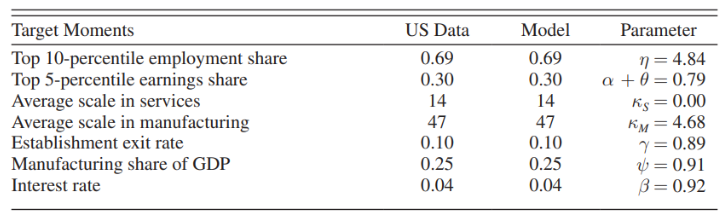
\includegraphics[width=0.8\linewidth]{pic/cali.png}
    \nonumber
    \label{fig:enter-label}
\end{figure}
根据论文中的结果:$\frac{\alpha}{\frac{1}{\eta}+\alpha+\theta}=0.3,\alpha+\theta=0.79$可得:$\alpha=0.3,\theta=0.49$
\subsection{基础模型:无固定成本、金融市场完备}
此时创业者可以选择利润的全局最优点,根据利润最大化问题:
$$\max_{k,l} \ \pi= z k^{\alpha} l^{\theta} - Rk - wl$$
得到一阶条件:由于目标函数是凹函数,一阶条件就是充要条件
$$\frac{d\pi}{dk}=\alpha z k^{\alpha-1} l^{\theta}-R=0$$
$$\frac{d\pi}{dk}=\theta z k^{\alpha} l^{\theta-1}-w=0$$
从而可以得到$\frac{w}{R}=\frac{\theta}{\alpha}(\frac{k^*}{l^*})$,$k^*=\left(((r+\delta)/\alpha z)(w\alpha/(r+\delta)\theta)^\theta\right)^{(1/(\alpha+\theta-1))}$
\subsubsection{导入包}
我们接下来导入必要的包进行后续的计算,它们的作用分别是:
\begin{itemize}
    \item timeit:计时、调试
    \item numpy:矩阵运算
    \item numba:编译加速
    \item matplotlib.pyplot:绘图
\end{itemize}
\begin{lstlisting}
# import packages
import timeit
import numpy as np
from numba import njit,prange
import matplotlib.pyplot as plt
\end{lstlisting}

\subsubsection{参数设置}
\begin{lstlisting}
# parameters setting
# tech
alpha=0.3
theta=0.49
fc_m=4.68
fc_s=0

# depreciation
delta=0.06

# describing the process for entrepreneurial talent
gamma=0.89
eta=4.84

# discount factor
beta=0.92

# relative risk aversion
sigma=1.5

# intratemporal elasticity of substitution
epsilon=1

# service share in consumption
psi=0.91

# capital state
kmin = 0
kmax = 150
n_k = 250
kgrid = np.linspace(kmin, kmax, n_k)
\end{lstlisting}

\subsubsection{随机性建模}
首先,我利用cipy.stats中的pareto包,通过离散化帕累托分布,生成指定范围内的离散能力值和对应的概率。
首先,根据帕累托分布的形状参数和给定的下、上边界,利用分位点函数生成等间距的能力值网格。
然后,计算每个离散区间的累积分布差值,并归一化以得到概率。最后,移除第一个网格点并返回剩余的能力值和对应的概率。
这些离散化结果可用于进一步的概率计算或模拟。
\begin{lstlisting}
# talent probability
from scipy.stats import pareto
def discrete_pareto(shape,lower_bound,upper_bound,grid_numder):
    ability=np.linspace(pareto.ppf(lower_bound,shape),pareto.ppf(upper_bound,shape),(grid_numder+1))  # 可以从60%开始取点,但是没改全!!!
    probability=np.diff(pareto.cdf(ability,shape)) / (upper_bound-lower_bound)
    zgrid = ability[1:]
    return zgrid,probability
\end{lstlisting}
接着,我依据马尔可夫过程的理论,建模能力跨期的转移过程:如果状态$j$不变,则概率为$\gamma+(1-\gamma)*p_z[j]$,否则为$(1-\gamma)p_z[i]$。基于这个思路,我创建了能力的转移概率矩阵。
\begin{lstlisting}
zgrid,p_z = discrete_pareto(4.84,0.6,0.995,40)
n_z = len(zgrid)
V0 = np.zeros((n_k, n_z))
P=np.zeros((n_z, n_z))
for i in range(n_z):
    for j in range(n_z):
        if j==i:
            P[i,j]=gamma+(1-gamma)*p_z[j]
        else:
            P[i,j]=(1-gamma)*p_z[j]
\end{lstlisting}
\subsubsection{定义基础函数}
\begin{lstlisting}
def u(c):
    if c > 0:
        res = (c**(1-sigma))/(1-sigma)
    else:
        res = -np.inf
    return res
if compile:
    u = njit(u)
    
def budget_worker(a, x, w, r):
    return w + (1+r)*a - x
if compile:
    budget_worker = njit(budget_worker)
    
def budget_entrepreneur(z_index, k, l, a , x , w, r):
    R = r + delta
    return zgrid[z_index]*(k**alpha)*(l**theta) + (1+r)*a - R*k - w*l - x
if compile:
    budget_entrepreneur = njit(budget_entrepreneur)
\end{lstlisting}
\subsubsection{工人的递归}
下面按照价值函数迭代法的思路,建模每次迭代过程中的优化搜索:
\begin{lstlisting}
def V_current_worker(k_next_index, k_index, z_index, V_next, w, r):
    c = budget_worker(kgrid[k_index], kgrid[k_next_index], w, r)
    EV = np.sum(P[z_index,:]*V_next[k_next_index,:]) # expectation
    res = u(c) + beta*(gamma*V_next[k_next_index,z_index]+(1-gamma)*EV)
    return res
if compile:
    V_current_worker = njit(V_current_worker)
    
def V_max_worker(k_index, z_index, k_start, V, w, r):
    V_max = -np.inf
    for j in range(k_start,n_k):
        k_next = kgrid[j]
        V_new=V_current_worker(j,k_index,z_index, V, w, r)
        if V_new > V_max:
            V_max = V_new
            g_k = k_next
            k_start = j
        else:break
    return V_max, g_k, k_start
if compile:
    V_max_worker = njit(V_max_worker)

def V_update_worker(V, w, r):
    V_new = np.zeros((n_k, n_z))
    g_new = np.zeros((n_k, n_z))
    for i_z in prange(n_z): 
        k_start = 0
        for i_k in range(n_k): # loop over all state k
            V_new[i_k, i_z], g_new[i_k, i_z] ,k_start= \
            V_max_worker(i_k, i_z,k_start,V,w,r)
    return V_new, g_new
if compile:
    V_update_worker = njit(V_update_worker, parallel=True)
\end{lstlisting}

接下来,我们假设所有个体选择作为工人,进行价值函数迭代。假设$w=0.9,r=0.05$,得到的结果如下:
\begin{lstlisting}
def V_iteration_worker(V_initial,tol,w,r):
    V = V_initial
    error = np.inf
    count = 0
    max_iter = 1000
    print_skip = 50
    while count < max_iter and error > tol:
        V_new, g_new = V_update_worker(V,w,r)
        error = np.max(np.abs(V_new - V))
        V = V_new
        count = count + 1
        if count % print_skip == 0:
            print(f"Error at iteration {count} is {error}.")
    if error > tol:
        print("Failed to converge!")
    else:
        print(f"\nConverged in {count} iterations.")
    return V_new, g_new

start_time = timeit.default_timer()
V_worker, g_worker = V_iteration_worker(V0,tol=1e-7,w=0.9,r=0.05)
print("The time difference is :", timeit.default_timer() - start_time)
\end{lstlisting}
\begin{figure}[h]
    \centering
    \nonumber
    \subfigure{
    \begin{minipage}[t]{0.45\linewidth}
    \centering
    \nonumber
    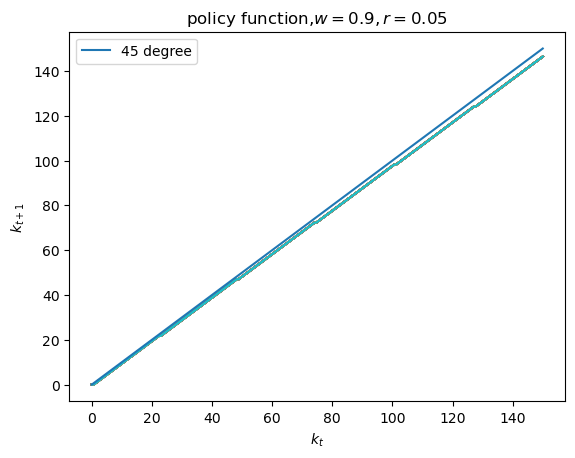
\includegraphics[width=2.5in]{pic/1.png}
    \end{minipage}}
    \subfigure{
    \begin{minipage}[t]{0.45\linewidth}
    \centering
    \nonumber
    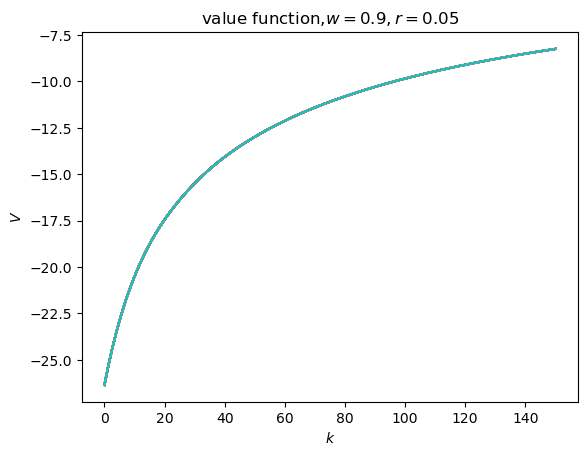
\includegraphics[width=2.5in]{pic/2.png}
    \end{minipage}}
\end{figure}

\subsubsection{创业者的递归}

\begin{lstlisting}
def V_current_entrepreneur(k_next_index, k_index, z_index, V_next, k, l, w, r):
    c = budget_entrepreneur(z_index, k, l, kgrid[k_index], \
        kgrid[k_next_index], w, r)
    EV = np.sum(P[z_index,:]*V_next[k_next_index,:]) 
    res = u(c) + beta*(gamma*V_next[k_next_index,z_index]+\
        (1-gamma)*EV)
    return res
if compile:
    V_current_entrepreneur = njit(V_current_entrepreneur)

def V_max_entrepreneur(k_index, z_index, k_start, V ,w, r):
    # R=r+delta
    k=(((r+delta)/alpha/zgrid[z_index])*(w*alpha/(r+delta)/theta)**theta)\
        **(1/(alpha+theta-1))
    l=k*(theta/alpha)*((r+delta)/w)
    V_max = -np.inf
    for j in range(k_start,n_k):
        k_next = kgrid[j]
        V_new=V_current_entrepreneur(j,k_index,z_index, V, k,l,w, r)
        if V_new > V_max:
            V_max = V_new
            g_k = k_next
            k_start = j
        else:break
    return V_max, g_k, k_start
if compile:
    V_max_entrepreneur = njit(V_max_entrepreneur)

def V_update_entrepreneur(V, w, r): # 冗余了
    V_new = np.zeros((n_k, n_z))
    g_new = np.zeros((n_k, n_z))
    for i_z in prange(n_z): 
        k_start = 0
        for i_k in range(n_k): # loop over all state k
            V_new[i_k, i_z], g_new[i_k, i_z] ,k_start= V_max_entrepreneur \
            (i_k, i_z,k_start, V, w, r)
    return V_new, g_new
if compile:
    V_update_entrepreneur = njit(V_update_entrepreneur, parallel=True)
\end{lstlisting}
接下来,我们假设所有个体选择创业,进行价值函数迭代。假设$w=0.9,r=0.05$,得到的结果如下:
\begin{lstlisting}
def V_iteration_entrepreneur(V_initial,tol,w,r):
    V = V_initial
    error = np.inf
    count = 0
    max_iter = 1000
    print_skip = 50
    while count < max_iter and error > tol:
        V_new, g_new = V_update_entrepreneur(V,w,r)
        error = np.max(np.abs(V_new - V))
        V = V_new
        count = count + 1
        if count % print_skip == 0:
            print(f"Error at iteration {count} is {error}.")
    if error > tol:
        print("Failed to converge!")
    else:
        print(f"\nConverged in {count} iterations.")
    return V_new, g_new

start_time = timeit.default_timer()
V_entrepreneur, g_entrepreneur = V_iteration_entrepreneur(V0,tol=1e-7,w=0.9,\
    r=0.05)
print("The time difference is :", timeit.default_timer() - start_time)
\end{lstlisting}
\begin{figure}[h]
    \centering
    \nonumber
    \subfigure{
    \begin{minipage}[t]{0.45\linewidth}
    \centering
    \nonumber
    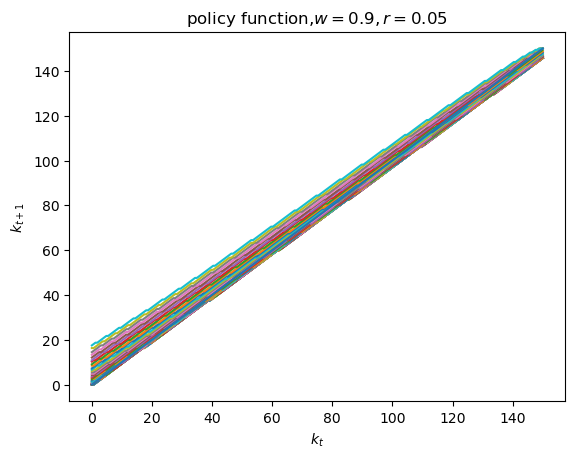
\includegraphics[width=2.5in]{pic/3.png}
    \end{minipage}}
    \subfigure{
    \begin{minipage}[t]{0.45\linewidth}
    \centering
    \nonumber
    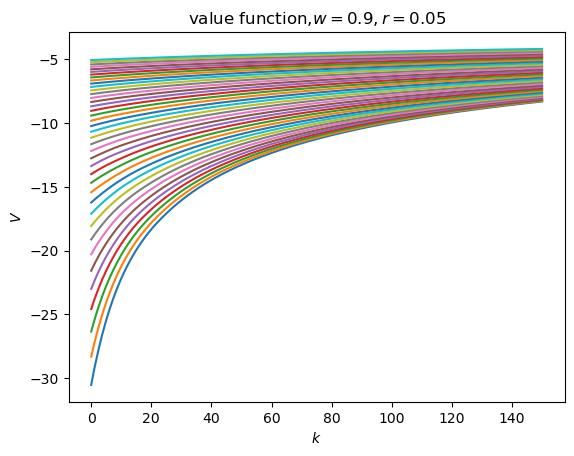
\includegraphics[width=2.5in]{pic/4.png}
    \end{minipage}}
\end{figure}
\subsubsection{职业选择:工人还是创业?个体问题的最优化}
首先,让我们将上面两个递归结果合并到一张图片上: 
\begin{figure}[h]
    \centering
    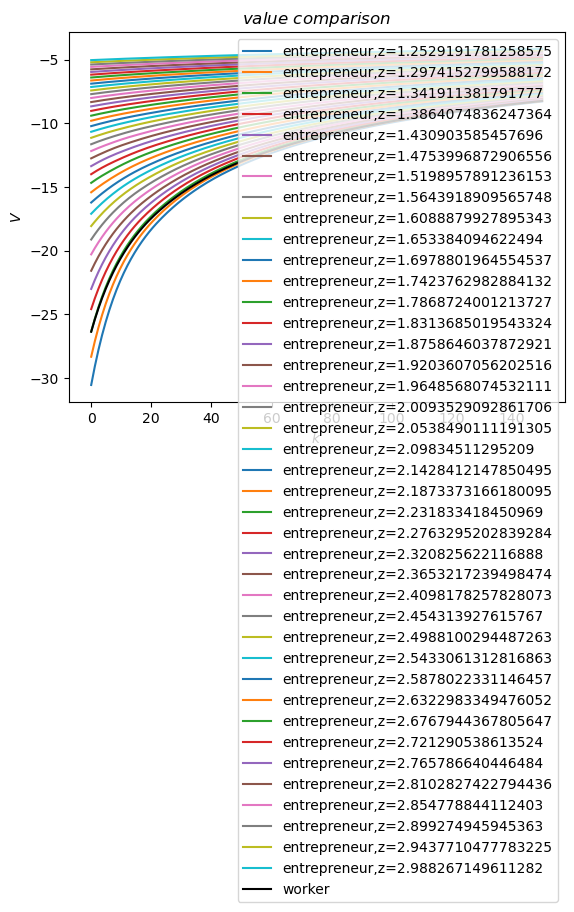
\includegraphics[width=0.5\linewidth]{pic/5.png}
    \nonumber
    \label{fig:enter-label}
\end{figure}
\\ 其中黑色线是工人的价值函数,可以看出,在某些状态下,创业是占优于做工人的。

由于个体问题的最优化要求比较不同职业选择下的效用大小,所以我在每次迭代时,对于每个状态,分别计算工人和创业者的效用,然后取较大值作为当前状态的效用,
并且取对应的对策函数为该状态的对策函数;同时我又引入了一个示性矩阵$state\_new$,如果在该状态个体选择创业,记为1。
接下来的更新迭代过程如下图所示:
\begin{figure}[h]
    \centering
    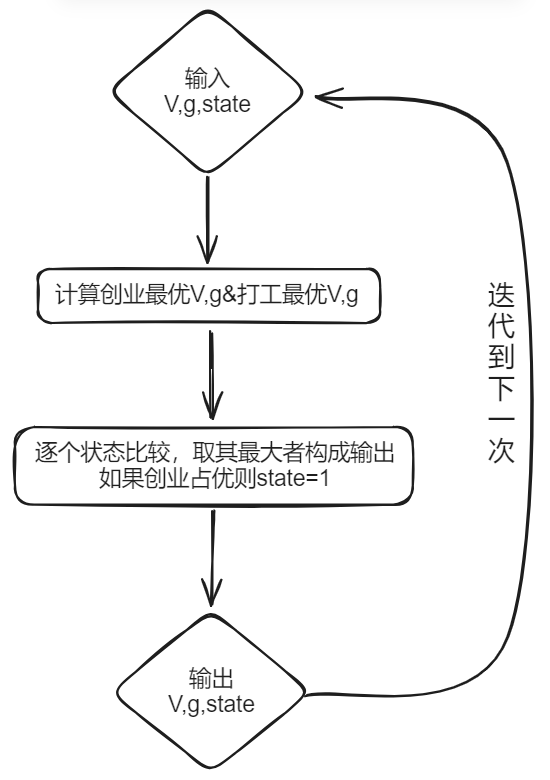
\includegraphics[width=0.5\linewidth]{pic/algorithm1.png}
    \nonumber
    \label{fig:enter-label}
\end{figure}
\begin{lstlisting}
def V_update(V, w, r): # 放到一起
    V_new = np.zeros((n_k, n_z))
    g_new = np.zeros((n_k, n_z))
    state_new = np.zeros((n_k, n_z))
    # V_worker,g_worker=V_update_worker(V, w, r)
    # V_entrepreneur,g_entrepreneur=V_update_entrepreneur(V, w, r)
    for i_z in prange(n_z):
        k_start_worker=0
        k_start_entrepreneur=0
        for i_k in range(n_k):
            V_new_worker, g_new_worker,k_start_worker= V_max_worker\
                (i_k, i_z,k_start_worker,V,w,r)
            V_new_entrepreneur, g_new_entrepreneur,k_start_entrepreneur= \
                V_max_entrepreneur(i_k, i_z,k_start_entrepreneur,V,w,r)
            if V_new_worker>=V_new_entrepreneur:
                V_new[i_k, i_z]=V_new_worker
                g_new[i_k, i_z]=g_new_worker
            else:
                V_new[i_k, i_z]=V_new_entrepreneur
                g_new[i_k, i_z]=g_new_entrepreneur
                state_new[i_k, i_z]=1
    return V_new, g_new, state_new
if compile:
    V_update = njit(V_update,parallel=True)


def V_iteration(V_initial,tol,w,r):
    V = V_initial
    error = np.inf
    count = 0
    max_iter = 1000
    while count < max_iter and error > tol:
        V_new, g_new, state_new = V_update(V, w, r)
        error = np.max(np.abs(V_new - V))
        V = V_new
        count = count + 1
    return V_new, g_new, state_new

start_time = timeit.default_timer()
V, g , state_entrepreneur= V_iteration(V0,tol=1e-7,w=0.9,r=0.05 )
print("The time difference is :", timeit.default_timer() - start_time)
\end{lstlisting}

最终合并递归的结果如下图:
\begin{figure}[h]
    \centering
    \nonumber
    \subfigure{
    \begin{minipage}[t]{0.45\linewidth}
    \centering
    \nonumber
    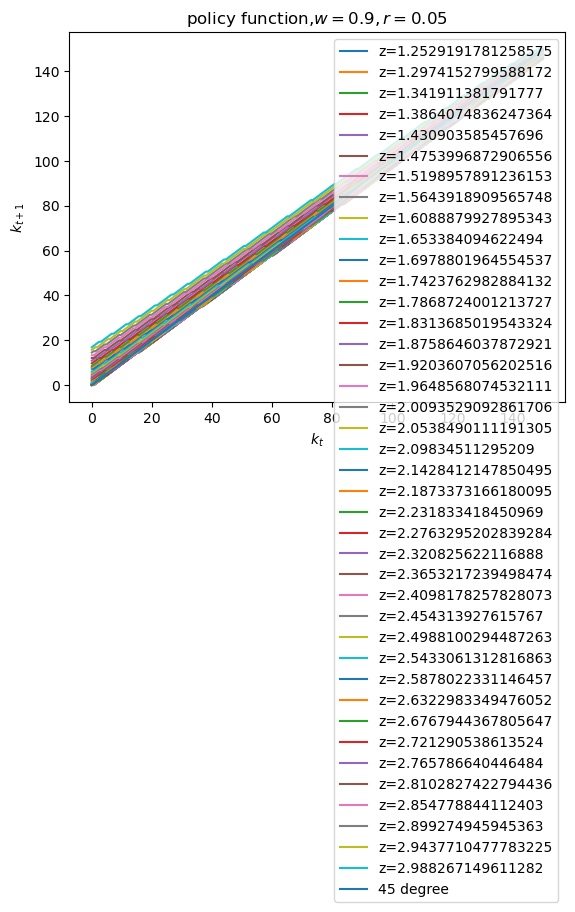
\includegraphics[width=2.5in]{pic/6.png}
    \end{minipage}}
    \subfigure{
    \begin{minipage}[t]{0.45\linewidth}
    \centering
    \nonumber
    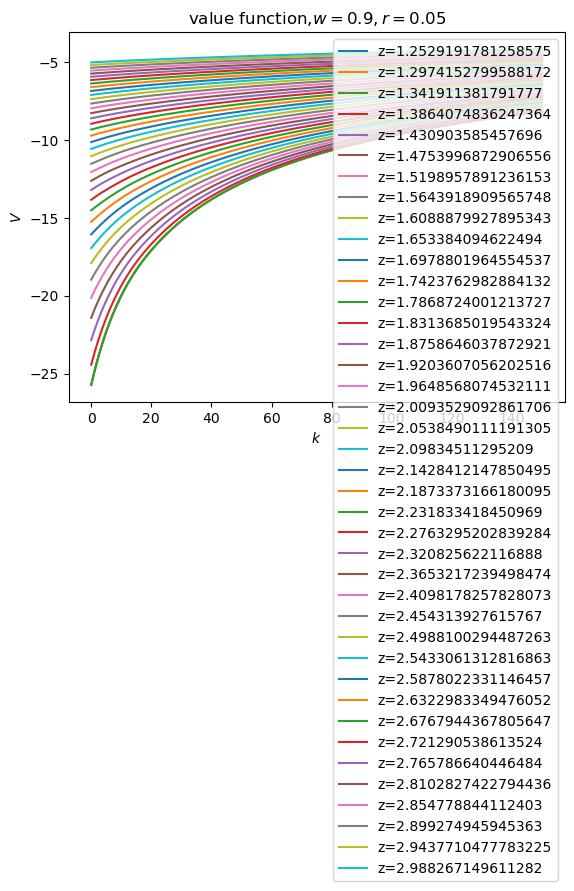
\includegraphics[width=2.5in]{pic/7.png}
    \end{minipage}}
\end{figure}
其中,在这个价格体系下,最终选择创业的状态有9250/10000个
\subsubsection{稳定分布的求解}
首先,我们要基于最终得到的对策函数生成状态$(a,\mathbf{z})$的转移概率矩阵。
由于大部分状态的转移概率为0,这个大矩阵是一个稀疏矩阵,所以我接下来用稀疏矩阵的形式表达转移概率矩阵,得到了`transQ\_sparse`函数。
`transQ\_sparse`函数将二维数组`g`转换为稀疏状态转移矩阵`Q`。它通过遍历状态空间中的每个状态,计算状态转移的目标索引和对应的转移概率,将这些信息存储在稀疏矩阵中。最终,函数利用这些数据构建并返回一个高效的压缩稀疏行(CSR)格式的状态转移矩阵。

\begin{lstlisting}
from scipy import sparse
def transQ_sparse(g):
    n_k, n_s = g.shape
    n = n_k * n_s
    row_indices = []
    col_indices = []
    values = []
    for j in numba.prange(n):
        i_k = j // n_s
        i_s = j % n_s
        diff = np.abs(g[i_k, i_s] - kgrid)
        mark = np.argmin(diff)
        j_prime_start = mark * n_s
        row = np.full(n_s, j)
        col = np.arange(j_prime_start, j_prime_start + n_s)
        val = P[i_s, :]
        row_indices.extend(row)
        col_indices.extend(col)
        values.extend(val)
    Q = sparse.csr_matrix((values, (row_indices, col_indices)), shape=(n, n))
    return Q
\end{lstlisting}

根据马尔可夫过程的性质,如果这个过程具有稳定分布$m^*$,那么对于任意分布$m:\lim_{n\to\infty}P^n m \to m^*$。
根据这一条件,我采用迭代的方法,让某一个分布$m$不断左乘转移矩阵,直到变化幅度小于一个外生给定的限度。
由于转移矩阵是一个稀疏矩阵,我接下来采用稀疏矩阵乘法进行迭代,以加快运算速度:
\begin{lstlisting}
import scipy.sparse as sp

def sparse_stationary_distribution_iteration(P, psi0, tol):
    P_csc = sp.csc_matrix(P.T)
    err = np.inf
    max_iter = 1000
    iter = 0
    print_skip = 50
    
    while iter < max_iter and err > tol:
        psi = P_csc.dot(psi0)
        err = np.max(np.abs(psi - psi0))
        iter = iter + 1
        psi0 = psi
        
    return psi0
\end{lstlisting}

\subsubsection{求解市场供求}
在得到了最终状态变量的稳定分布后,我们可以求出此时的市场供求大小,计算思路如下:
\begin{itemize}
    \item 信贷市场:根据资本的稳定边缘分布得到信贷供给;根据创业者的最优资本需求以概率为权重加总得到信贷需求;
    \item 劳动力市场:根据$1-state_new$得到工人的规模,从而得到劳动供给;根据创业者的最优劳动力需求以概率为权重加总得到劳动力需求
\end{itemize}
\begin{lstlisting}
    # Compute Demand and Supply in Capital Market
    def capital_and_labor(w,r):
        V0 = np.zeros((n_k, n_z))
        V_new,g,state_entrepreneur=V_iteration(V0,1e-7,w,r)
        Q=transQ_sparse(g)
        psi0 = np.ones((n_k * n_z))/(n_k * n_z)
        ss=sparse_stationary_distribution_iteration(Q,psi0,10e-5)
        # ss=stationary_distribution(Q)
        tmp = ss.reshape((n_k, n_z))
        a_dist=capital_marginal(ss)
        z_dist=state_marginal(ss)
    ## capital_supply
        capital_supply=np.dot(kgrid,a_dist)
    ## labor_supply
        state_worker=np.ones((n_k, n_z))-state_entrepreneur
        labor_supply_joint=np.zeros((n_k, n_z))            
    ## capital_demand & labor_demand
        R=r+delta
        capital_demand_joint= np.zeros((n_k, n_z))
        labor_demand_joint= np.zeros((n_k, n_z))
        for i_k in range(n_k):
            for i_z in range(n_z):
                capital_demand_joint[i_k,i_z]=state_entrepreneur[i_k,i_z]*\
                    ((R/alpha/zgrid[i_z])*(w*alpha/R/theta)**theta)\
                    **(1/(alpha+theta-1))*tmp[i_k,i_z] 
                #capital_demand_joint 这里已经乘以概率了
                labor_demand_joint[i_k,i_z]=capital_demand_joint[i_k,i_z]*\
                    (theta/alpha)*(R/w)
                labor_supply_joint[i_k,i_z]=state_worker[i_k,i_z]*tmp[i_k,i_z]
        labor_supply=np.sum(labor_supply_joint)
        capital_demand=np.sum(capital_demand_joint)
        labor_demand=np.sum(labor_demand_joint)
        
        return capital_supply,capital_demand,labor_supply,labor_demand
\end{lstlisting}

\subsubsection{画图,确定均衡价格范围}
\begin{lstlisting}
### plot market curves
from tqdm import tqdm

def labor_curve(wmin, wmax, wgrid_number,r):
    wgrid = np.linspace(wmin, wmax, wgrid_number)
    l_supply = np.zeros(wgrid_number)
    l_demand = np.zeros(wgrid_number)
    for i in tqdm(range(wgrid_number)):
        w0 = wgrid[i]
        capital_supply,capital_demand,l_supply[i],l_demand[i]=\
            capital_and_labor(w0,r)
    return wgrid, l_supply, l_demand

wgrid, labor_supply, labor_demand = labor_curve(
    wmin=0.5, wmax=1.5, wgrid_number=50,r=0.082
)
# Plot
plt.scatter(labor_supply,wgrid,label="labor_supply")
plt.scatter(labor_demand,wgrid,label="labor_demand")
plt.ylabel('w')
plt.xlabel('labor')
plt.legend()
plt.grid(True)
\end{lstlisting}

\begin{figure}[h]
    \centering
    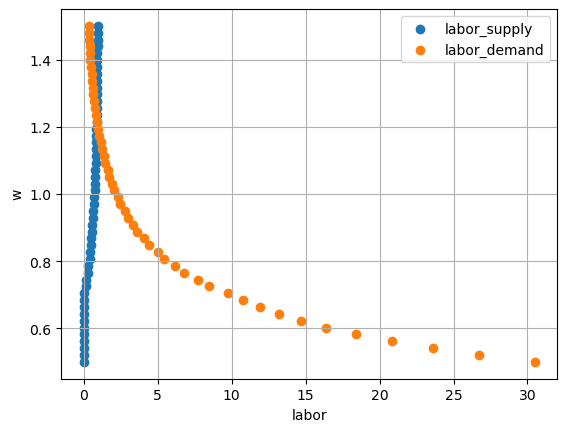
\includegraphics[width=0.8\linewidth]{pic/8.png}
    \nonumber
    \label{fig:enter-label}
\end{figure}

接下来,为了画出资本市场的供求曲线,我们需要保证给定利率时劳动力市场是出清的,所以首先定义局部均衡(劳动力市场)价格搜索函数:
\begin{lstlisting}
def equilibrium_k(w,r):
    a_supply,a_demand,l_supply,l_demand=capital_and_labor(w,r)
    res_k=a_supply-a_demand
    print('w=',w,'r=,',r,'capital supply=',a_supply,'capital demand=',\
        a_demand,'res_k=',res_k)
    return res_k
    
def equilibrium_l(w,r):
    a_supply,a_demand,l_supply,l_demand=capital_and_labor(w,r)
    res_l=l_supply-l_demand
    print('w=',w,'r=,',r,'labor supply=',l_supply,'labor demand=',\
        l_demand,'res_l=',res_l)
    return res_l

import scipy.optimize as optimize
def w_update(r):
    wmax=0.5
    wmin=1.5
    start_time = timeit.default_timer()
    solution = optimize.root_scalar(
    f=equilibrium_l, bracket=[wmin,wmax], args=(r), method="bisect", xtol=1e-5
    )
    print("The time difference is :", timeit.default_timer() - start_time)
    print("final w=", solution.root)
    return solution.root
\end{lstlisting}

在此基础上,我们绘制出资本市场曲线:
\begin{lstlisting}
from tqdm import tqdm

def capital_curve(rmin, rmax, rgrid_number):
    rgrid = np.linspace(rmin, rmax, rgrid_number)
    a_supply = np.zeros(rgrid_number)
    a_demand = np.zeros(rgrid_number)
    for i in tqdm(range(rgrid_number)):
        r0 = rgrid[i]
        w = w_update(r0)
        a_supply[i],a_demand[i],l_supply,l_demand=capital_and_labor(w,r0)
    return rgrid, a_supply, a_demand

rgrid, capital_supply, capital_demand = capital_curve(
    rmin=0.03, rmax=0.082, rgrid_number=20
)
\end{lstlisting}
\begin{figure}[h]
    \centering
    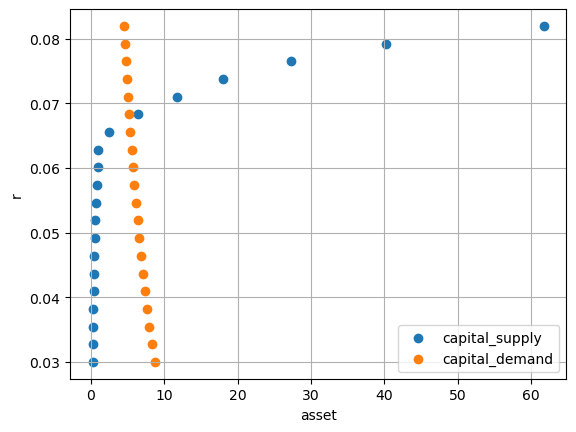
\includegraphics[width=0.8\linewidth]{pic/9.png}
    \nonumber
    \label{fig:enter-label}
\end{figure}

\newpage

\subsubsection{嵌套二分法搜索均衡价格$(w,r)$}
接下来,我按照下图的思路,设计嵌套二分法搜索算法:

\begin{figure}[ht]
    \centering
    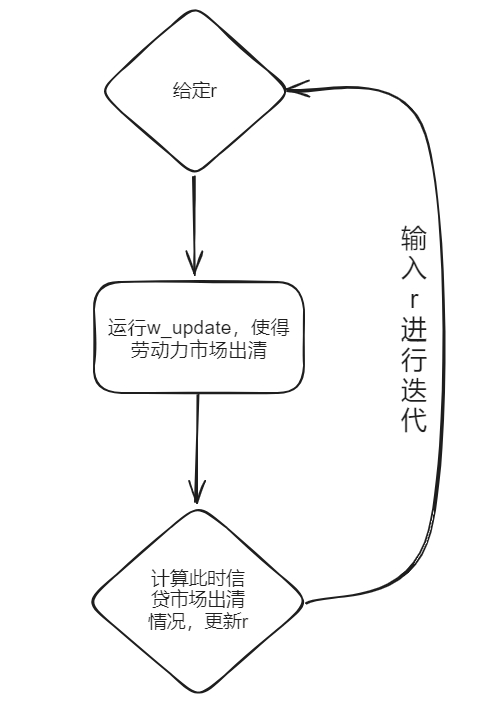
\includegraphics[width=0.35\linewidth]{pic/algor4.png}
    \nonumber
    \label{fig:enter-label}
\end{figure}

\begin{lstlisting}
def rw_iteration(tol):
    rmin= 0.06557895
    rmax=0.06831579
    r0=1/2*(rmin+rmax)
    error = np.inf
    count = 0
    max_iter = 1000
    print_skip = 50
    while count < max_iter and error > tol:
        w = w_update(r0)
        res_k = equilibrium_k(w,r0)
        if res_k < 0:
            rmin=r0
        else:
            rmax=r0
        r0 = 1/2*(rmin+rmax)
        error = np.abs(rmax-rmin)
        count = count + 1
        print('rmin=',rmin,'rmax=',rmax,'r=',r0,'iteration times=',count)
    if error > tol:
        print("Failed to converge!")
    else:
        print(f"\nConverged in {count} iterations.")
    return r0 

r_eq = rw_iteration(1e-5)
w_eq = w_update(r_eq)
\end{lstlisting}

\begin{figure}[h]
    \centering
    \nonumber
    \subfigure{
    \begin{minipage}[t]{0.45\linewidth}
    \centering
    \nonumber
    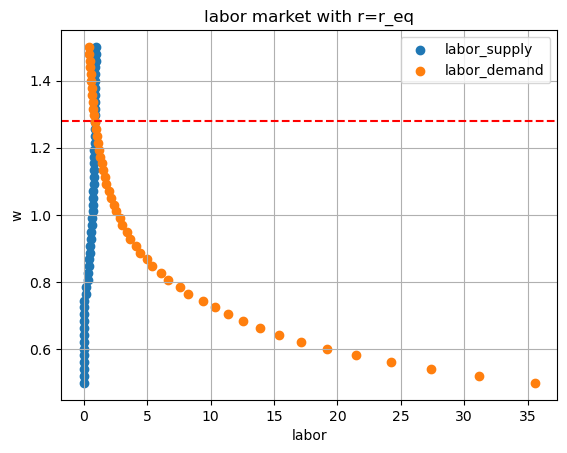
\includegraphics[width=2.5in]{pic/10.png}
    \end{minipage}}
    \subfigure{
    \begin{minipage}[t]{0.45\linewidth}
    \centering
    \nonumber
    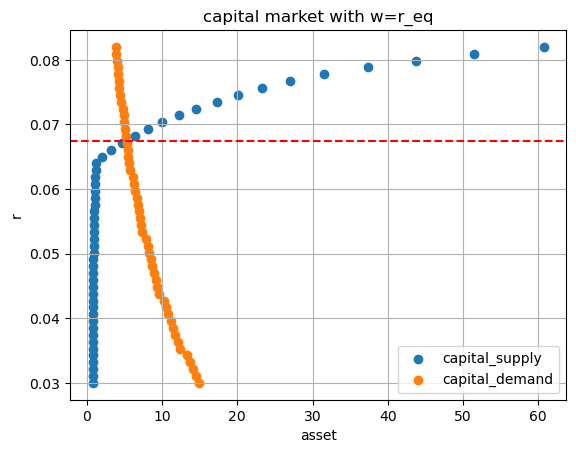
\includegraphics[width=2.5in]{pic/11.png}
    \end{minipage}}
\end{figure}

w= 1.2784652709960938 r=, 0.0673669831640625 labor supply= 0.8601581137047082 labor demand= 0.8601536854748624 res\_l= 4.428229845809817e-06

w= 1.2784652709960938 r=, 0.0673669831640625 capital supply= 5.286293284979713 capital demand= 5.286074773600964 res\_k= 0.00021851137874939752


\subsubsection{检验:制造品市场出清情况}
接下来,按照瓦尔拉斯定律,我们检验制造品市场出清情况以确定社会是否达到竞争性均衡,制造品供求计算思路如下:
\begin{itemize}
    \item 制造品供给:选择创业个体对应的产出结果,以概率为权重求和
    \item 制造品需求:计算个体的预算结余,以概率为权重求和;基于信贷市场计算资本折旧。
\end{itemize}
\begin{lstlisting}
def goods(w,r):
    R = r+delta
    V0 = np.zeros((n_k, n_z))
    V_new,g,state_entrepreneur=V_iteration(V0,1e-7,w,r)
    state_worker=np.ones((n_k , n_z))-state_entrepreneur
    Q=transQ_sparse(g)
    psi0 = np.ones((n_k * n_z))/(n_k * n_z)
    ss=sparse_stationary_distribution_iteration(Q,psi0,10e-5)
    tmp = ss.reshape((n_k, n_z))
    a_dist=capital_marginal(ss)
    z_dist=state_marginal(ss)
    goods_demand_joint = np.zeros((n_k, n_z))
    goods_supply_joint = np.zeros((n_k, n_z))
    capital_joint = np.zeros((n_k,n_z))        
    for i_k in range(n_k):
        for i_z in range(n_z):
            k = ((R / alpha / zgrid[i_z]) * (w * alpha / R / theta) ** theta) ** (1 / (alpha + theta - 1))
            l = k * (theta / alpha) * (R / w)
            goods_demand_joint[i_k,i_z]=(state_entrepreneur[i_k,i_z]*budget_entrepreneur(i_z,k,l,kgrid[i_k], g[i_k,i_z], w, r)+state_worker[i_k,i_z]*budget_worker(kgrid[i_k], g[i_k,i_z], w, r))*tmp[i_k,i_z]
            goods_supply_joint[i_k,i_z]=state_entrepreneur[i_k,i_z]*(zgrid[i_z]*(k**alpha)*(l**theta))*tmp[i_k,i_z]
            capital_joint[i_k,i_z]=state_entrepreneur[i_k,i_z]*k*tmp[i_k,i_z]
    goods_demand = np.sum(goods_demand_joint)
    goods_supply = np.sum(goods_supply_joint)
    capital = np.sum(capital_joint)
    return goods_supply,goods_demand,capital
\end{lstlisting}

goods supply= 2.2442379889773636 goods demand= 1.932168152755912 capital supply= 5.286293284979713 res\_m = -0.005107760877331224
\subsection{拓展:引入固定成本}
\subsubsection{均衡结果}
相对于模型一,我们引入了固定成本,唯一的改变就是在计算创业者收入约束时加入了固定成本。变为
$$f(z_{index}, k, l) + (1+r)*a - R*k - w*l - a' - (1+r)*\kappa_m$$
\begin{lstlisting}
def budget_entrepreneur(z_index, k, l, a , x , w, r): # add fixed cost fc_m
    R = r + delta
    return f(z_index, k, l) + (1+r)*a - R*k - w*l - x - (1+r)*fc_m
if compile:
    budget_entrepreneur = njit(budget_entrepreneur)
\end{lstlisting}


我采用了和第一个模型一样的状态设定,最终得到的均衡结果如下:
\begin{figure}[h]
    \centering
    \nonumber
    \subfigure{
    \begin{minipage}[t]{0.45\linewidth}
    \centering
    \nonumber
    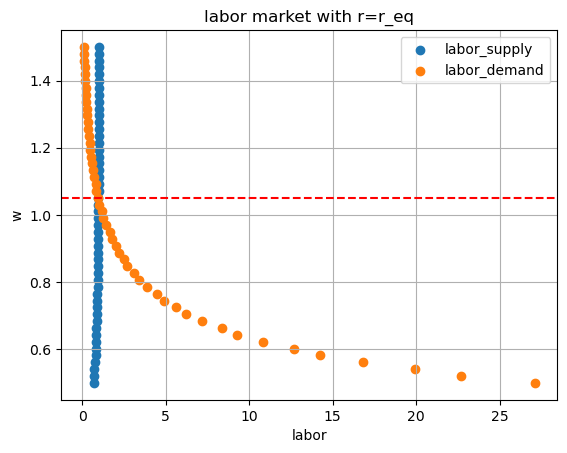
\includegraphics[width=2.5in]{pic/12.png}
    \end{minipage}}
    \subfigure{
    \begin{minipage}[t]{0.45\linewidth}
    \centering
    \nonumber
    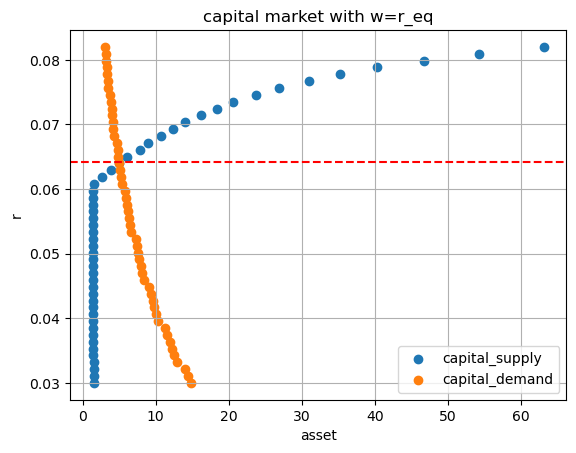
\includegraphics[width=2.5in]{pic/13.png}
    \end{minipage}}
\end{figure}

w= 1.0506057739257812 r=, 0.0641437126171875 labor supply= 0.9606730031352523 labor demand= 0.9606527637272572 res\_l= 2.0239407995115144e-05

w= 1.0506057739257812 r=, 0.0641437126171875 capital supply= 4.958073945660268 capital demand= 4.9774472404158425 res\_k= -0.019373294755574477

与第一个模型相比可以发现均衡的工资和利率都减小了,因为此时创业个体减少,劳动力和资本需求都减少,从而市场价格下降。
\subsubsection{检验:制造品市场出清情况}
接下来,按照瓦尔拉斯定律,我们检验制造品市场出清情况以确定社会是否达到竞争性均衡,制造品供求计算思路如下:
\begin{itemize}
    \item 制造品供给:选择创业个体对应的产出结果,以概率为权重求和
    \item 制造品需求:计算个体的预算结余,以概率为权重求和;基于信贷市场计算资本折旧;选择创业个体的固定成本
\end{itemize}
\begin{lstlisting}
def goods(w,r):
    R = r+delta
    V0 = np.zeros((n_k, n_z))
    V_new,g,state_entrepreneur=V_iteration(V0,1e-7,w,r)
    state_worker=np.ones((n_k , n_z))-state_entrepreneur
    Q=transQ_sparse(g)
    psi0 = np.ones((n_k * n_z))/(n_k * n_z)
    ss=sparse_stationary_distribution_iteration(Q,psi0,10e-5)
    tmp = ss.reshape((n_k, n_z))
    a_dist=capital_marginal(ss)
    z_dist=state_marginal(ss)
    goods_demand_joint = np.zeros((n_k, n_z))
    goods_supply_joint = np.zeros((n_k, n_z))
    capital_joint = np.zeros((n_k,n_z))        
    fixed_cost_joint = np.zeros((n_k,n_z))      
    for i_k in range(n_k):
        for i_z in range(n_z):
            k = ((R / alpha / zgrid[i_z]) * (w * alpha / R / theta) ** theta)\
                 ** (1 / (alpha + theta - 1))
            l = k * (theta / alpha) * (R / w)
            goods_demand_joint[i_k,i_z]=(state_entrepreneur[i_k,i_z]*budget_\
                entrepreneur(i_z,k,l,kgrid[i_k], g[i_k,i_z], w, r)+\
                state_worker[i_k,i_z]\
                *budget_worker(kgrid[i_k], g[i_k,i_z], w, r))*tmp[i_k,i_z]
            goods_supply_joint[i_k,i_z]=state_entrepreneur[i_k,i_z]*\
                (zgrid[i_z]*(k**alpha)*(l**theta))*tmp[i_k,i_z]
            capital_joint[i_k,i_z]=state_entrepreneur[i_k,i_z]*k*tmp[i_k,i_z]
            fixed_cost_joint[i_k,i_z]=state_entrepreneur[i_k,i_z]*\
            tmp[i_k,i_z]*fc_m
    goods_demand = np.sum(goods_demand_joint)
    goods_supply = np.sum(goods_supply_joint)
    capital = np.sum(capital_joint)
    fixed_cost = np.sum(fixed_cost_joint)
    return goods_supply,goods_demand,capital,fixed_cost
\end{lstlisting}

goods supply= 2.0597292659379907 goods demand= 1.569439130946358 capital supply= 4.9774472404158425 fixed cost= 0.18405034532703038 res\_m=-0.004212717218099432
\subsection{拓展:引入固定成本、不完备金融市场}
\subsubsection{创业者重新建模}
由于此时信贷市场的不完善,创业者可能无法选择到全局最优的资本水平,甚至可能无法进行创业。

对此,我们需要进一步分析一下激励相容条件:
$$\max_l \{ p_jz_jf(k,l)-wl \} -Rk-(1+r)p_j \kappa_j+(1+r)a \geq (1-\phi)[\max_l \{ p_jz_jf(k,l)-wl \}+(1-\delta)k]$$
我们移项可以得到:
$$\phi \max_l \{ p_jz_jf(k,l)-wl \} -Rk-(1+r)p_j \kappa_j+(1+r)a - (1-\phi)(1-\delta)k\geq 0$$
对于$\max_l \{ p_jz_jf(k,l)-wl \}$这一部分,我们可以求出$l^*(k)=(\frac{\theta z k^\alpha}{w})^{1/(1-\theta)}$。
从而左式可以视为$g(a,\mathbf{z};k)$的函数,且关于$k$是凹的,给定$(a,\mathbf{z})$,左式具有全局最大值点$k_{max}=\left( \frac{(r + \delta) + (1 - \delta)(1 - \phi)}{\left( \phi w \left( \frac{\theta z}{w} \right)^{\frac{1}{1 - \theta}} \right) \frac{\alpha}{\theta}} \right)^{\frac{1}{\left( \frac{\alpha}{1 - \theta} \right) - 1}}$。依据这些性质,我们可以得到求解创业者资本需求的思路:

\begin{figure}[h]
    \centering
    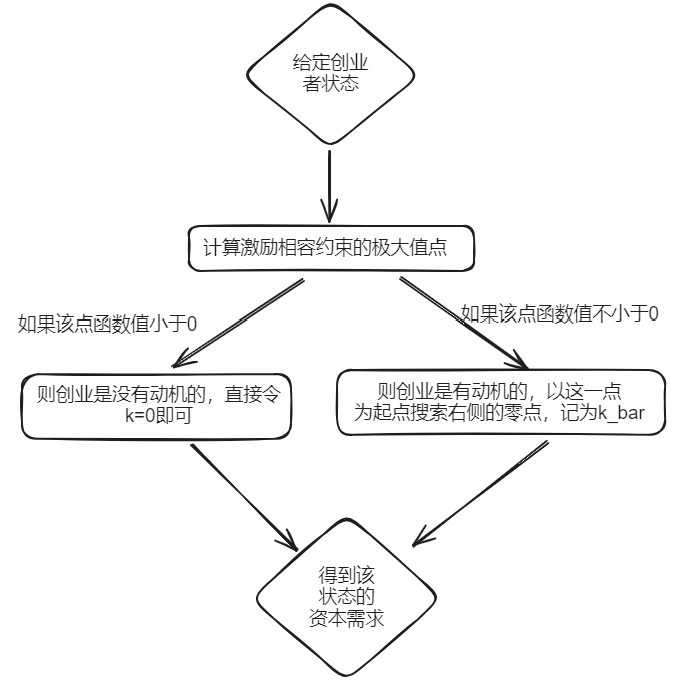
\includegraphics[width=0.8\linewidth]{pic/algor2.png}
    \nonumber
    \label{fig:enter-label}
\end{figure}

只不过需要注意的是,求解激励相容边界的过程用到了scipy\_optimize,无法进行njit编译加速,所以我事先算好激励相容边界,
然后将其作为参数输入到编译加速的主体代码部分,得到创业者的资本需求和对应的劳动力需求。

\begin{lstlisting}
def capital_bound_matrix(w, r):
    bound_matrix = np.zeros((n_k, n_z))
    for i_k in range(n_k):
        for i_z in range(n_z):
            z_index = i_z
            a_index = i_k
            k_max = (((r+delta)+(1-delta)*(1-phi))/((phi*w*(theta*zgrid\ 
                [z_index]/w)**(1/(1-theta)))*alpha/theta))**(1/((alpha/(1-theta))-1))
            res = capital_constraint(k_max, z_index, a_index , w, r)
            if res < 0 :
                bound_matrix[i_k,i_z]=0
            if res == 0 :
                bound_matrix[i_k,i_z]=k_max
            if res > 0 :
                solution = brentq(capital_constraint, k_max,1e+10, args=\ 
                (z_index, a_index, w, r))
                bound_matrix[i_k,i_z] = solution
            # print(k_max,res)
    return  bound_matrix

@njit
def capital_opt_unconditional(k_index, z_index, w, r):
    R = r + delta
    opt = ((R / alpha / zgrid[z_index]) * (w * alpha / (R * theta))\
         ** theta) ** (1 / (alpha + theta - 1))
    return opt

@njit
def capital_demand(k_index, z_index, w, r, bound_matrix): # KKT
    if bound_matrix[k_index, z_index] > capital_opt_unconditional\
        (k_index, z_index, w, r):
        k_demand = capital_opt_unconditional(k_index, z_index, w, r)
    else:
        k_demand = bound_matrix[k_index, z_index]
    return k_demand

@njit
def capital_opt_matrix(w, r):
    R = r + delta
    capital_matrix = np.zeros((n_k, n_z))
    for i_k in range(n_k):
        for i_z in range(n_z):
            capital_matrix[i_k, i_z] = capital_opt_unconditional(i_k, i_z, w, r)
    return capital_matrix


@njit
def V_current_entrepreneur(k_next_index, k_index, z_index, V_next, \
    w, r, bound_matrix):
    R = r + delta
    k = capital_demand(k_index, z_index, w, r, bound_matrix)
    l = (theta*zgrid[z_index]*(k**alpha)/w)**(1/(1-theta))
    c = budget_entrepreneur(z_index, k, l, kgrid[k_index], \
        kgrid[k_next_index], w, r)
    EV = np.sum(P[z_index, :] * V_next[k_next_index, :])  # expectation
    if k==0: # 此时没有动机创业,默认为0效用
        res = 0
    res = u(c) + beta * (gamma * V_next[k_next_index, z_index] + \
        (1 - gamma) * EV)

    return res

@njit
def V_max_entrepreneur(k_index, z_index, k_start, V, w, r, bound_matrix):
    V_max = -np.inf
    for j in range(k_start, n_k):
        k_next = kgrid[j]
        V_new = V_current_entrepreneur(j, k_index, z_index, V, \
            w, r, bound_matrix)
        if V_new > V_max:
            V_max = V_new
            g_k = k_next
            k_start = j
        else:
            break
    return V_max, g_k, k_start
\end{lstlisting}

\subsubsection{个体设定}
此时由于借贷的难度进一步增大,为了保证最后模型有个体创业,我将社会总体的创业能力状态的上限和个人储蓄的上限提高:
\begin{lstlisting}
kmin =0
kmax =250
n_k = 250
kgrid = np.linspace(kmin, kmax, n_k)
zgrid,p_z = discrete_pareto(4.84,0.6,0.9995,40)
n_z = len(zgrid)
V0 = np.zeros((n_k, n_z))
P=np.zeros((n_z, n_z))
for i in range(n_z):
    for j in range(n_z):
        if j==i:
            P[i,j]=gamma+(1-gamma)*p_z[j]
        else:
            P[i,j]=(1-gamma)*p_z[j]
\end{lstlisting}

\newpage

\subsubsection{均衡结果}
\begin{figure}[h]
    \centering
    \nonumber
    \subfigure{
    \begin{minipage}[t]{0.45\linewidth}
    \centering
    \nonumber
    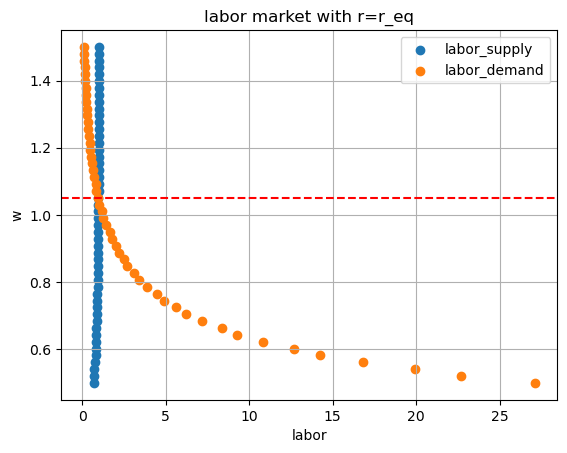
\includegraphics[width=2.5in]{pic/14.png}
    \end{minipage}}
    \subfigure{
    \begin{minipage}[t]{0.45\linewidth}
    \centering
    \nonumber
    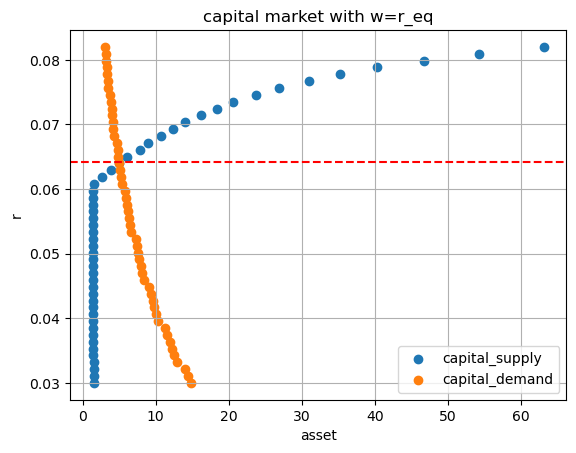
\includegraphics[width=2.5in]{pic/15.png}
    \end{minipage}}
\end{figure}

w= 1.2001914978027344 r= 0.0542102196875 labor suply= 0.9803610043496709 labor demand= 1.0649923109827002 res\_l= -0.08463130663302931

w= 1.2001914978027344 r= 0.0542102196875 capital supply= 6.533385159801248 capital demand= 6.1637618367606155 res\_k= 0.3696233230406323

\subsubsection{检验:制造品市场出清情况}
同理第二个模型的算法,我检验了此时制造品市场出清情况,结果如下:
\\ goods demand= 1.5643896244668494 goods supply= 2.6195000097174486 capital supply= 6.613677358910731 capital demand= 6.192661207367035 labor supply= 0.9801264837152996 labor demand= 1.0694585048397978 fixed cost= 0.09300805621243344
res\_m=0.5602397003435385

\newpage

\section{论文复现第二阶段:两部门模型}
\subsection{个体设定}
此时的消费变为$(c_S,c_m)$,效用函数发生了变化。由于$\varepsilon=1$,所以效用函数退化为了Cobb-Douglas形式:

$$
u(c_S,c_m)=\frac{1}{1-\sigma}(c_S^\psi c_m^{1-\psi})^{1-\sigma}
$$

给定总消费$c$,消费者的最优消费为:

$$
c_S=c\left(p_s+\frac{(1-\phi)(1-\sigma)}{\phi(1-\sigma)}\right)^{-1},c_m=c_s \frac{(1-\phi)(1-\sigma)}{\phi(1-\sigma)}
$$



此时个体的状态变量为$(a;z_s,z_m)$,其中$z_s,z_m$相互独立,所以需要平行建立两个
Pareto概率分布,并将其相乘联合。此时的转移概率建模如下:

我们构造一个大小为 \(n_s \times n_m\) 的状态转移概率矩阵 \(P\)。对于每个状态 \(i\) 和 \(j\),矩阵元素 \(P[i, j]\) 表示从状态 \(i\) 转移到状态 \(j\) 的概率。矩阵的构造基于以下规则:

\begin{itemize}
    \item 如果 \(j = i\),则
    \[
    P[i, j] = \gamma + (1-\gamma) \cdot ps[j_s] \cdot pm[j_m]
    \]
    \item 如果 \(j \neq i\),则
    \[
    P[i, j] = (1-\gamma) \cdot ps[j_s] \cdot pm[j_m]
    \]
\end{itemize}

其中,\(j_s\) 和 \(j_m\) 分别是 \(j\) 在 \(n_s\) 和 \(n_m\) 维度上的索引:

\[
j_s = j \mod n_s
\]
\[
j_m = \left\lfloor \frac{j}{n_s} \right\rfloor
\]

同时,为了保证有人储蓄进行创业,我们在此也提升了个人储蓄的上限。
\begin{lstlisting}
kmin = 0
kmax = 250
n_k = 250
kgrid = np.linspace(kmin, kmax, n_k)
sgrid,ps = discrete_pareto(4.84,0.6,0.99,5)
mgrid,pm = discrete_pareto(4.84,0.6,0.9995,20)
# mgrid,p_m = discrete_pareto(4.84,0.6,0.99,20)
n_s = len(sgrid)
n_m = len(mgrid)
V0 = np.zeros((n_k, n_s*n_m))
# joint ditribution (p_s,p_m)
P=np.zeros((n_s*n_m, n_s*n_m))
for i in range(n_s*n_m):
    for j in range(n_s*n_m):
        j_s = j % n_s
        j_m = j // n_s
        if j==i:
            P[i,j]=gamma+(1-gamma)*ps[j_s]*pm[j_m]
        if j!=i:
            P[i,j]=(1-gamma)*ps[j_s]*pm[j_m]
\end{lstlisting}

\subsection{迭代算法思路}
延续第三个模型,在第四个模型只需要平行添加一个服务业创业的迭代,图示如下:
\begin{figure}[h]
    \centering
    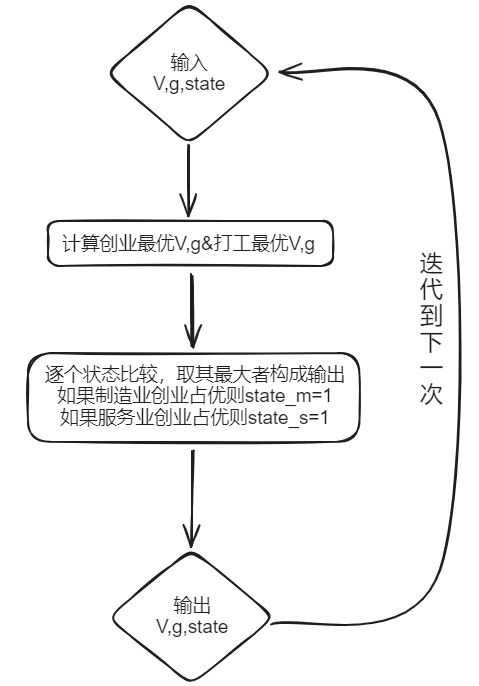
\includegraphics[width=0.4\linewidth]{pic/algor3.png}
    \nonumber
    \label{fig:enter-label}
\end{figure}

\begin{lstlisting}
def u(c_s,c_m):
    c = c_s + c_m
    if c > 0:
        # res = (1/(1-sigma))*(psi*c_s**(1-1/epsilon)+(1-psi)*c_m**\
            (1-1/epsilon))**((1-sigma)/(1-1/epsilon))
        res = (1/(1-sigma))*(((c_s)**psi+(c_m)**(1-psi))**(1-sigma))
    else:
        res = -np.inf
    return res
if compile:
    u = njit(u)

def budget_worker(a, x, w, r):
    return w + (1+r)*a - x
if compile:
    budget_worker = njit(budget_worker)

## service
def f_s(z_index, k, l):
    i_s = z_index % n_s
    f = sgrid[i_s]*(k**alpha)*(l**theta)
    return f
if compile:
    f_s = njit(f_s)

@njit
def budget_s(z_index, k, l, a , x , w, r):
    R = r + delta
    return f_s(z_index, k, l) + (1+r)*a - R*k - w*l - x - (1+r)*fc_s

@njit
def capital_constraint_s(k, z_index, a_index , w, r):
    R=r+delta
    i_s = z_index % n_s
    f=phi*(1/theta-1)*w*(theta*sgrid[i_s]*k**alpha/w)**(1/(1-theta))+\
        (1+r)*kgrid[a_index]-R*k-(1+r)*fc_s-(1-phi)*(1-delta)*k
    return f


## manufacture
def f_m(z_index, k, l):
    i_m = z_index // n_s
    f = mgrid[i_m]*(k**alpha)*(l**theta)
    return f
if compile:
    f_m = njit(f_m)

@njit
def budget_m(z_index, k, l, a , x , w, r):
    R = r + delta
    return f_m(z_index, k, l) + (1+r)*a - R*k - w*l - x - (1+r)*fc_m

@njit
def capital_constraint_m(k, z_index, a_index , w, r):
    R=r+delta
    i_m = z_index // n_s
    f=phi*(1/theta-1)*w*(theta*mgrid[i_m]*k**alpha/w)**(1/(1-theta))+\
        (1+r)*kgrid[a_index]-R*k-(1+r)*fc_m-(1-phi)*(1-delta)*k
    return f

\end{lstlisting}

\begin{lstlisting}   
# worker
def V_current_worker(k_next_index, k_index, z_index, V_next, w, r, p_s):
    c = budget_worker(kgrid[k_index], kgrid[k_next_index], w, r)
    c_s = c*(p_s+(1-psi)*(1-sigma)/(psi*(1-sigma)))**(-1)
    c_m = c_s*(1-psi)*(1-sigma)/(psi*(1-sigma))
    EV = np.sum(P[z_index,:]*V_next[k_next_index,:]) # expectation
    res = u(c_s,c_m) + beta*(gamma*V_next[k_next_index,z_index]\    
        +(1-gamma)*EV)
    return res
if compile:
    V_current_worker = njit(V_current_worker)

def V_max_worker(k_index, z_index, k_start, V, w, r, p_s):
    V_max = -np.inf
    for j in range(k_start,n_k):
        k_next = kgrid[j]
        V_new=V_current_worker(j,k_index,z_index, V, w, r, p_s)
        if V_new > V_max:
            V_max = V_new
            g_k = k_next
            k_start = j
        else:break
    return V_max, g_k, k_start
if compile:
    V_max_worker = njit(V_max_worker)

def V_update_worker(V, w, r, p_s):
    V_new = np.zeros((n_k, n_s*n_m))
    g_new = np.zeros((n_k, n_s*n_m))
    for i_z in prange(n_s*n_m): 
        k_start = 0
        for i_k in range(k_start,n_k): # loop over all state k
            V_new[i_k, i_z], g_new[i_k, i_z] ,k_start= \
                V_max_worker(i_k,i_z,k_start,V,w,r,p_s)
    return V_new, g_new
if compile:
    V_update_worker = njit(V_update_worker, parallel=True)


    # worker
    def V_current_worker(k_next_index, k_index, z_index, V_next, w, r, p_s):
        c = budget_worker(kgrid[k_index], kgrid[k_next_index], w, r)
        c_s = c*(p_s+(1-psi)*(1-sigma)/(psi*(1-sigma)))**(-1)
        c_m = c_s*(1-psi)*(1-sigma)/(psi*(1-sigma))
        EV = np.sum(P[z_index,:]*V_next[k_next_index,:]) 
        res = u(c_s,c_m) + beta*(gamma*V_next\  
            [k_next_index,z_index]+(1-gamma)*EV)
        return res
    if compile:
        V_current_worker = njit(V_current_worker)
    
    def V_max_worker(k_index, z_index, k_start, V, w, r, p_s):
        V_max = -np.inf
        for j in range(k_start,n_k):
            k_next = kgrid[j]
            V_new=V_current_worker(j,k_index,z_index, V, w, r, p_s)
            if V_new > V_max:
                V_max = V_new
                g_k = k_next
                k_start = j
            else:break
        return V_max, g_k, k_start
    if compile:
        V_max_worker = njit(V_max_worker)
    
    def V_update_worker(V, w, r, p_s):
        V_new = np.zeros((n_k, n_s*n_m))
        g_new = np.zeros((n_k, n_s*n_m))
        for i_z in prange(n_s*n_m): 
            k_start = 0
            for i_k in range(k_start,n_k): # loop over all state k
                V_new[i_k, i_z], g_new[i_k, i_z] ,k_start= \
                    V_max_worker(i_k,i_z,k_start,V,w,r,p_s)
        return V_new, g_new
    if compile:
        V_update_worker = njit(V_update_worker, parallel=True)
\end{lstlisting}

\begin{lstlisting}
def m_capital_bound_matrix(w, r):
    bound_matrix = np.zeros((n_k, n_s*n_m))
    for a_index in range(n_k):
        for z_index in range(n_s*n_m):
            i_m = z_index // n_s
            k_max = (((r+delta)+(1-delta)*(1-phi))/((phi*w*\
                (theta*mgrid[i_m]/w)**(1/(1-theta)))*alpha/theta))\
                **(1/((alpha/(1-theta))-1))
            res = capital_constraint_m(k_max, z_index, a_index , w, r)
            if res < 0 :
                bound_matrix[a_index,z_index]=0
            if res == 0 :
                bound_matrix[a_index,z_index]=k_max
            if res > 0 :
                solution = brentq(capital_constraint_m, k_max,1e+10,\
                     args=(z_index, a_index, w, r))
                bound_matrix[a_index,z_index] = solution
            # print(k_max)
    return  bound_matrix
    
def s_capital_bound_matrix(w, r):
    bound_matrix = np.zeros((n_k, n_s*n_m))
    for a_index in range(n_k):
        for z_index in range(n_s*n_m):
            i_s = z_index % n_s
            k_max = (((r+delta)+(1-delta)*(1-phi))/((phi*w*\
                (theta*sgrid[i_s]/w)**(1/(1-theta)))*alpha/theta))\
                **(1/((alpha/(1-theta))-1))
            res = capital_constraint_s(k_max, z_index, a_index , w, r)
            if res < 0 :
                bound_matrix[a_index,z_index]=0
            if res == 0 :
                bound_matrix[a_index,z_index]=k_max
            if res > 0 :
                solution = brentq(capital_constraint_s, k_max,1e+10,\
                 args=(z_index, a_index, w, r))
                bound_matrix[a_index,z_index] = solution
            # print(k_max)
    return  bound_matrix
\end{lstlisting}

\begin{lstlisting}
# service
@njit
def s_capital_opt_unconditional(k_index, z_index, w, r):
    R = r + delta
    i_s = z_index % n_s
    opt = ((R / alpha / sgrid[i_s]) * (w * alpha / R / theta) ** theta)\
         ** (1 / (alpha + theta - 1))
    return opt

@njit
def s_capital_demand(k_index, z_index, w, r, bound_matrix):
    if bound_matrix[k_index, z_index] > s_capital_opt_unconditional\
        (k_index, z_index, w, r):
        capital_demand = s_capital_opt_unconditional(k_index,\
             z_index, w, r)
    else:
        capital_demand = bound_matrix[k_index, z_index]
    return capital_demand


@njit
def s_V_current_entrepreneur(k_next_index, k_index, z_index, \
    V_next, w, r,  p_s, bound_matrix):
    R = r + delta
    i_s = z_index % n_s
    # k_matrix = s_capital_demand_matrix(w, r, bound_matrix)
    k = s_capital_demand(k_index, z_index, w, r, bound_matrix)
    l = (theta*sgrid[i_s]*(k**alpha)/w)**(1/(1-theta))
    c = budget_s(z_index, k, l, kgrid[k_index], kgrid[k_next_index], w, r)
    c_s = c*(p_s+(1-psi)*(1-sigma)/(psi*(1-sigma)))**(-1)
    c_m = c_s*(1-psi)*(1-sigma)/(psi*(1-sigma))
    EV = np.sum(P[z_index, :] * V_next[k_next_index, :])  # expectation
    res = u(c_s,c_m) + beta * (gamma * V_next[k_next_index, z_index]\
         + (1 - gamma) * EV)
    return res

@njit
def s_V_max_entrepreneur(k_index, z_index, k_start, V, w, \
    r, p_s, bound_matrix):
    V_max = -np.inf
    for j in range(k_start, n_k):
        k_next = kgrid[j]
        V_new = s_V_current_entrepreneur(j, k_index, z_index, V, \
            w, r, p_s, bound_matrix)
        if V_new > V_max:
            V_max = V_new
            g_k = k_next
            k_start = j
        else:
            break
    return V_max, g_k, k_start
\end{lstlisting}

\begin{lstlisting}
# manufacture
@njit
def m_capital_opt_unconditional(k_index, z_index, w, r):
    R = r + delta
    i_m = z_index // n_s
    opt = ((R / alpha / mgrid[i_m]) * (w * alpha / R / theta)\
         ** theta) ** (1 / (alpha + theta - 1))
    return opt

@njit
def m_capital_demand(k_index, z_index, w, r, bound_matrix):
    if bound_matrix[k_index, z_index] > \
        m_capital_opt_unconditional(k_index, z_index, w, r):
        capital_demand = m_capital_opt_unconditional\
            (k_index, z_index, w, r)
    else:
        capital_demand = bound_matrix[k_index, z_index]
    return capital_demand

@njit
def m_V_current_entrepreneur(k_next_index, k_index, z_index,\
     V_next, w, r,  p_s, bound_matrix):
    R = r + delta
    i_m = z_index // n_s
    # k_matrix = m_capital_demand_matrix(w, r, bound_matrix)
    k = m_capital_demand(k_index, z_index, w, r, bound_matrix)
    l = (theta*mgrid[i_m]*(k**alpha)/w)**(1/(1-theta))
    c = budget_m(z_index, k, l, kgrid[k_index], kgrid[k_next_index], w, r)
    c_s = c*(p_s+(1-psi)*(1-sigma)/(psi*(1-sigma)))**(-1)
    c_m = c_s*(1-psi)*(1-sigma)/(psi*(1-sigma))
    EV = np.sum(P[z_index, :] * V_next[k_next_index, :])  # expectation
    res = u(c_s,c_m) + beta * (gamma * \
        V_next[k_next_index, z_index] + (1 - gamma) * EV)
    return res

@njit
def m_V_max_entrepreneur(k_index, z_index, k_start, V, w, r, p_s, bound_matrix):
    V_max = -np.inf
    for j in range(k_start, n_k):
        k_next = kgrid[j]
        V_new = m_V_current_entrepreneur(j, k_index, z_index, V, w,\
             r, p_s, bound_matrix)
        if V_new > V_max:
            V_max = V_new
            g_k = k_next
            k_start = j
        else:
            break
    return V_max, g_k, k_start
\end{lstlisting}

\begin{lstlisting}
def V_update(V, w, r, p_s, bound_matrix_s, bound_matrix_m):
    V_new = np.zeros((n_k, n_s*n_m))
    g_new = np.zeros((n_k, n_s*n_m))
    state_manufacture = np.zeros((n_k, n_s*n_m))
    state_service = np.zeros((n_k, n_s*n_m))
    for i_z in prange(n_s*n_m):
        k_start_worker=0
        k_start_manufacture=0
        k_start_service=0
        for i_k in range(n_k):
            V_new_worker, g_new_worker,k_start_worker= \
                V_max_worker(i_k, i_z, k_start_worker, V, w, r, p_s)
            V_new_manufacture, g_new_manufacture,k_start_manufacture= \
                m_V_max_entrepreneur(i_k, i_z, k_start_manufacture, V, w,\
                r, p_s, bound_matrix_m)
            V_new_service, g_new_service,k_start_service= \
                s_V_max_entrepreneur(i_k, i_z, k_start_service,\
                V, w, r, p_s, bound_matrix_s)
            if V_new_service> V_new_manufacture and V_new_service \
                > V_new_worker:
                V_new[i_k, i_z]=V_new_service
                g_new[i_k, i_z]=g_new_service
                state_service[i_k, i_z]=1
            if V_new_manufacture > V_new_service and V_new_manufacture \
                > V_new_worker:
                V_new[i_k, i_z]=V_new_manufacture
                g_new[i_k, i_z]=g_new_manufacture
                state_manufacture[i_k, i_z]=1
            else:
                V_new[i_k, i_z]=V_new_worker
                g_new[i_k, i_z]=g_new_worker
    return V_new, g_new, state_manufacture, state_service
if compile:
    V_update = njit(V_update,parallel=True)

def V_iteration(V_initial,tol,w,r,p_s, bound_matrix_s, bound_matrix_m):
    V = V_initial
    error = np.inf
    count = 0
    max_iter = 1000
    while count < max_iter and error > tol:
        V_new, g_new, state_manufacture, state_service = \
            V_update(V, w, r,p_s, bound_matrix_s, bound_matrix_m)
        error = np.max(np.abs(V_new - V))
        V = V_new
        count = count + 1
        # if count % print_skip == 0:
            # print(f"Error at iteration {count} is {error}.")
    return V_new, g_new, state_manufacture , state_service
\end{lstlisting}

\subsection{求解市场供求}
在得到了最终状态变量的稳定分布后,我们可以求出此时的市场供求大小,计算思路如下:
\begin{itemize}
    \item 信贷市场:根据资本的稳定边缘分布得到信贷供给;根据创业者(服务业和制造业)的最优资本需求以概率为权重加总得到信贷需求;
    \item 劳动力市场:根据$1-state_{manufacture}-state_{service}$得到工人的规模,从而得到劳动供给;根据创业者(服务业和制造业)的最优劳动力需求以概率为权重加总得到劳动力需求
    \item 服务品市场:根据创业者(服务业)的生产函数求解每个状态的供给,然后以概率为权重求和;根据个体的预算约束求解总消费,再根据最优服务品消费的一阶条件求解服务品需求,然后以概率为权重求和
\end{itemize}
\begin{lstlisting}
# Compute Demand and Supply in Capital Market
def capital_and_labor_and_service(w,r,p_s):
    # initialize
    # start_time = timeit.default_timer()
    bound_matrix_s = s_capital_bound_matrix(w,r)
    bound_matrix_m = m_capital_bound_matrix(w,r)
    V0 = np.zeros((n_k, n_s*n_m))
    # iteration
    V_new,g,state_manufacture,state_service=V_iteration(V0,1e-7,w,r,\
        p_s,bound_matrix_s,bound_matrix_m)
    # stable distribution
    Q=transQ_sparse(g)
    psi0 = np.ones((n_k * n_s*n_m))/(n_k * n_s*n_m)
    ss=sparse_stationary_distribution_iteration(Q,psi0,1e-4)
    tmp = ss.reshape((n_k, n_s*n_m))
    # a_dist=capital_marginal(ss)
    # compute demand and supply
    # capital_supply=np.dot(kgrid,a_dist)
    state_worker=np.ones((n_k, n_s*n_m))\
        -state_manufacture-state_service
    R=r+delta
    # l = np.sum(state_worker*tmp)
    capital_supply_joint= np.zeros((n_k, n_s*n_m))
    capital_demand_joint= np.zeros((n_k, n_s*n_m))
    labor_supply_joint=np.zeros((n_k, n_s*n_m))
    labor_demand_joint= np.zeros((n_k, n_s*n_m))
    service_demand_joint = np.zeros((n_k, n_s*n_m))
    service_supply_joint = np.zeros((n_k, n_s*n_m))
    for i_k in range(n_k):
        for i_z in range(n_s*n_m):
            capital_supply_joint[i_k,i_z]=tmp[i_k,i_z]\
                *g[i_k,i_z]
            labor_supply_joint[i_k,i_z] = \
                state_worker[i_k,i_z]*tmp[i_k,i_z]
            i_s = i_z % n_s
            i_m = i_z // n_s
            k_m=m_capital_demand(i_k, i_z, w, r, bound_matrix_m)\
                *state_manufacture[i_k,i_z]
            k_s=s_capital_demand(i_k, i_z, w, r, bound_matrix_s)\
                *state_service[i_k,i_z]
            capital_demand_joint[i_k,i_z] = (k_m+k_s)*tmp[i_k,i_z]
            l_m = (theta*mgrid[i_m]*(k_m**alpha)/w)**(1/(1-theta))
            l_s = (theta*sgrid[i_s]*(k_s**alpha)/w)**(1/(1-theta))
            labor_demand_joint[i_k,i_z] = (l_m+l_s)*tmp[i_k,i_z]
            # service_demand_joint[i_k,i_z]=\
                budget_worker(kgrid[i_k], g[i_k,i_z], w, r)*\
                ((p_s+((1-psi)/psi))**(-1))*tmp[i_k,i_z]
            service_demand_joint[i_k,i_z]=((p_s+((1-psi)/psi))**(-1))\
                *tmp[i_k,i_z]*(budget_worker(kgrid[i_k], g[i_k,i_z], w, r)\
                *state_worker[i_k,i_z]+budget_s(i_z,k_s,l_s,kgrid[i_k],\
                g[i_k,i_z],w,r)*state_service[i_k,i_z]+budget_m(i_z,k_m,\
                l_m,kgrid[i_k],g[i_k,i_z],w,r)*state_manufacture[i_k,i_z])
            service_supply_joint[i_k,i_z]=state_service[i_k,i_z]*tmp[i_k,i_z]\
                *f_s(i_z,k_s,l_s)
    capital_supply=np.sum(capital_supply_joint)
    labor_supply=np.sum(labor_supply_joint)
    k_demand=np.sum(capital_demand_joint)
    l_demand=np.sum(labor_demand_joint)
    service_demand=np.sum(service_demand_joint)
    service_supply=np.sum(service_supply_joint)
    return capital_supply,k_demand,labor_supply,l_demand,\
        service_supply,service_demand
\end{lstlisting}

\subsubsection{求解均衡}
沿用前面的思路,采用三重嵌套法进行搜索
\begin{enumerate}
    \item 给定$(r,p_s)$,搜索$w^*$使得劳动力市场出清
    \item 基于$(w^*,p_s)$求解资本市场出清情况,更新$r$,直到资本市场出清,记此时利率为$r^*$
    \item 给定$(w^*,r^*)$求解服务品市场出清情况,更新$p_s$,回到第一步,迭代直到服务品市场出清。
\end{enumerate}

\begin{lstlisting}
def equilibrium_k(w,r,p_s):
    a_supply,a_demand,l_supply,l_demand,s_supply,s_demand=\
        capital_and_labor_and_service(w,r,p_s)
    res_k=a_supply-a_demand
    print('w=',w,'r=',r,'p_s=',p_s,'capital supply=',a_supply,\
        'capital demand=',a_demand,'res_k=',res_k)
    return res_k
    
def equilibrium_l(w,r,p_s):
    a_supply,a_demand,l_supply,l_demand,s_supply,s_demand=\
        capital_and_labor_and_service(w,r,p_s)
    res_l=l_supply-l_demand
    print('w=',w,'r=',r,'p_s=',p_s,'labor suply=',l_supply,\
        'labor demand=',l_demand,'res_l=',res_l)
    return res_l

def equilibrium_s(w,r,p_s):
    a_supply,a_demand,l_supply,l_demand,s_supply,s_demand=\
        capital_and_labor_and_service(w,r,p_s)
    res_s=s_supply-s_demand
    print('w=',w,'r=',r,'p_s=',p_s,'service suply=',s_supply,\
        'service demand=',s_demand,'res_s=',res_s)
    return res_s
\end{lstlisting}

\begin{lstlisting}
def w_update(r,p_s,tol):
    wmax=1.6
    wmin=1.2
    w0=1/2*(wmin+wmax)
    error = np.inf
    count = 0
    max_iter = 1000
    print_skip = 50
    while count < max_iter and error > tol:
        res = equilibrium_l(w0,r,p_s)
        if res < 0:
            wmin=w0
        else:
            wmax=w0
        w0=1/2*(wmin+wmax)
        error = np.abs(wmax-wmin)
        count = count + 1
    if error > tol:
        print("Failed to converge!")
    else:
        print(f"\nConverged in {count} iterations.")
    print("final w=", w0)
    return w0

def r_update(p_s,tol):
    rmin=0.056
    rmax=0.0755
    r0=1/2*(rmin+rmax)
    error = np.inf
    count = 0
    max_iter = 1000
    while count < max_iter and error > tol:
        w = w_update(r0,p_s,1e-4)
        res_k = equilibrium_k(w,r0,p_s)
        if res_k < 0:
            rmin=r0
        else:
            rmax=r0
        r0 = 1/2*(rmin+rmax)
        error = np.abs(rmax-rmin)
        count = count + 1
    if error > tol:
        print("Failed to converge!")
    else:
        print(f"\nConverged in {count} iterations.")
    return r0
\end{lstlisting}

\begin{lstlisting}
def p_iteration(tol):
    pmin=1
    pmax=2
    p0=0.5*(pmin+pmax)
    error = np.inf
    count = 0
    max_iter = 1000
    while count < max_iter and error > tol:
        r = r_update(p0,1e-4)
        w = w_update(r,p0,1e-4)
        res = equilibrium_s(w,r,p0)
        if res > 0:
            pmax = p0
        else:
            pmin = p0
        p0=0.5*(pmin+pmax)
        error = np.abs(pmax-pmin)
        count = count + 1
        print('pmin=',pmin,'pmax=',pmax,'p0=',p0,'r=',r,'w=',w,\
            'iteration times=',count,'res=',res)
    if error > tol:
        print("Failed to converge!")
    else:
        print(f"\nConverged in {count} iterations.")
    return p0
\end{lstlisting}

\begin{lstlisting}
ps_eq = p_iteration(1e-4)
r_eq = r_update(ps_eq,1e-5)
w_eq = w_update(r_eq,ps_eq,1e-5)
\end{lstlisting}

\subsection{均衡结果}
w= 1.491937255859375 r= 0.067067138671875 p\_s= 1.47802734375

\begin{figure}[h]
    \centering
    \nonumber
    \subfigure{
    \begin{minipage}[t]{0.32\linewidth}
    \centering
    \nonumber
    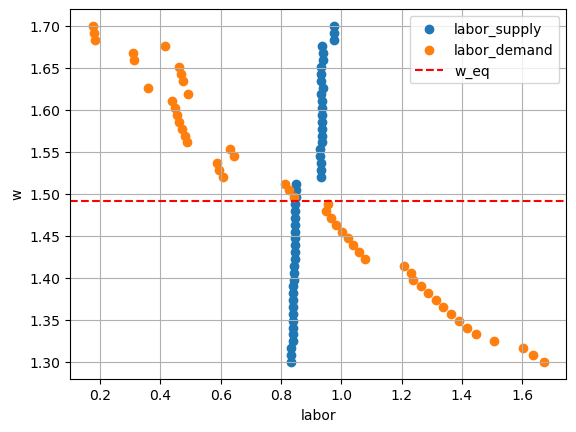
\includegraphics[width=2in]{pic/16.png}
    \caption*{劳动力市场}
    \end{minipage}}
    \subfigure{
    \begin{minipage}[t]{0.32\linewidth}
    \centering
    \nonumber
    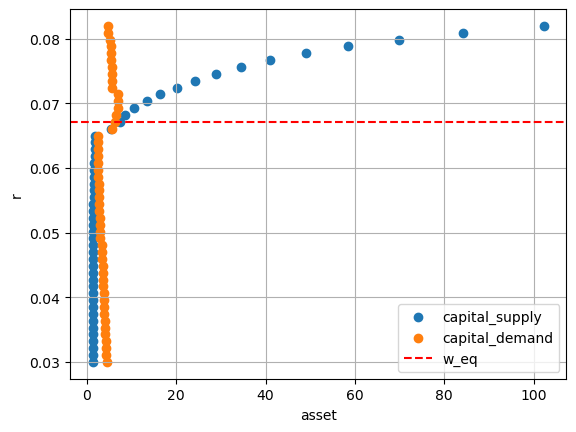
\includegraphics[width=2in]{pic/17.png}
    \caption*{信贷市场}
    \end{minipage}}
    \subfigure{
    \begin{minipage}[t]{0.32\linewidth}
    \centering
    \nonumber
    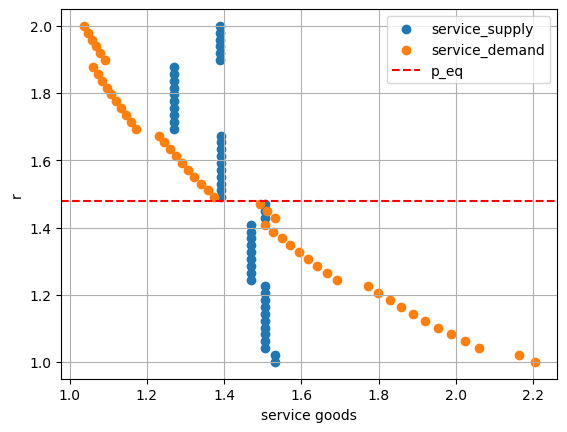
\includegraphics[width=2in]{pic/18.png}
    \caption*{服务品市场}
    \end{minipage}}
\end{figure}

w= 1.4919342041015624 r= 0.067067138671875 p\_s= 1.47802734375 \\labor suply= 0.8468278230983346 labor demand= 0.9455805231953405 res\_l= -0.09875270009700587

w= 1.4919342041015624 r= 0.067067138671875 p\_s= 1.47802734375 \\capital supply= 7.352796837845994 capital demand= 6.399414886188415 res\_k= 0.9533819516575788

w= 1.4919342041015624 r= 0.067067138671875 p\_s= 1.47802734375 \\service suply= 1.5056943948722066 service demand= 1.4841182367893744 res\_s= 0.021576158082832197

\subsection{检验:制造品市场出清情况}
下面检验制造品市场的出清情况:
\begin{enumerate}
    \item 制造品供给:选择创业(制造业)的个体的产出,以概率为权重求和
    \item 制造品需求:基于服务品需求计算个体的制造品需求,以概率为权重求和;以及资本的折旧
\end{enumerate}
最终的计算结果如下:
\\ m-goods\_demand= 0.1467809245176304 m-goods\_supply= 1.37337484040816 capital\_supply= 7.352796837845994 capital\_demand= 6.399414886188415 fixed cost= 0.0717415018857231 res\_m=0.7088731064785485

\end{document}
